\section{Mockups}
Um allen Projektbeteiligten ein Bild der zukünftigen Applikation zu vermitteln, sind für die wichtigsten Seiten Mockups entstanden. In diesem Abschnitt wird auf zwei Ansichten in der Connection Verwaltung eingegangen. Alle anderen Mockups sind im Anhang auf der Seite \pageref{Mockups} ersichtlich.\\
Weiter konnte dank der Mockups diverse nicht angedachte Use Cases und Features ermittelt werden.
\subsubsection{Connection Übersicht}
\begin{figure}[H]
	\centering
	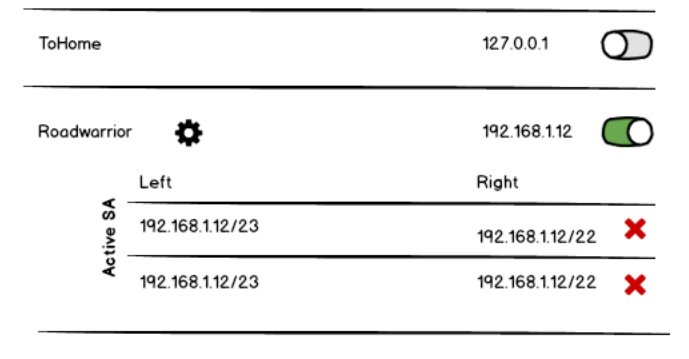
\includegraphics[width=330pt]{images/mockups/short_con_overview.jpg}
	\caption{Ausschnitt aus der Connection Übersicht}
\end{figure}
\medskip
Die erstellten Verbindungen werden in Zeilenform untereinander angeordnet. Es gibt einen zentralen Toggle Button, der die Verbindung aktiviert/deaktiviert und gleichzeitig den Verbindungsstatus anzeigt. 
Nach dem eine Verbindung gestartet und diese erfolgreich aufgebaut wurde, erweitert sich die Ansicht und es werden Statusinformationen angezeigt.

\subsubsection{Connection hinzufügen}
\noindent\begin{minipage}[t]{0.55\textwidth}
\vspace{0pt}
    \begin{figure}[H]
    	\centering
    	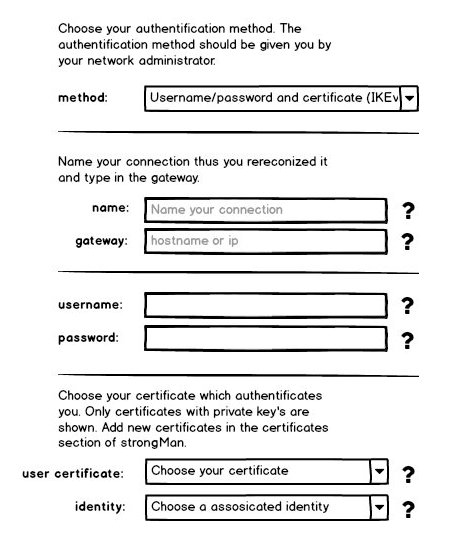
\includegraphics[width=240pt]{images/mockups/short_con_config.jpg}
    	\caption{Ausschnitt aus dem Connection hinzufügen}
    \end{figure}
\end{minipage}
\hfill
\begin{minipage}[t]{0.45\textwidth}
\vspace{0pt}
Nachdem der Benutzer die Authentifizierungsmethod ausgewählt hat (hier nicht ersichtlich), erscheinen unterhalb die entsprechenden Eingabefelder.

Das Konfigurieren einer Verbindung wird so einfach wie möglich gestaltet. Der Benutzer soll kurz vor jeder Eingabe informiert werden, welchen Nutzen das entsprechende Feld hat und sich bei Schwierigkeiten an den Hilfetexten orientieren können (Klick auf die Fragezeichen).
\end{minipage}